\section{Expected Sensitivity to Appearance}

\label{subsec:fitter}
\subsection{Fitting Code}
\improvement{Maybe all of this oscfit stuff should just be moved to just before the systematics section.}

Checks in this analysis are first performed using solely simulation files.
In order to understand the expected sensitivity of this analysis, \improvement{should i even talk about oscfit itself? it seems a bit awkward} {a fitting package previously used to fit the $\nu_\mu$ disappearance} \findref{msu and desy disappearance}.
The code, known as \emph{OscFit}, works in multiple stages. \needfig{Flowchart of oscfit fitting. at least broadly}
After separating the simulation into separate channels consisting of $\nu_e^{CC}$, $\nu_\mu^{CC}$, $\nu_\tau^{CC}$, $\nu^{NC}$, $\mu_{atm}$, and accidental triggers, the analytic systematics are applied.
These systematics solely rely on information about the particle interaction in order to calculate correction factors to the event weights and are not sensitive to the order of application.
The oscillation calculations are performed at this stage and are based on the Prob3++ code \findref{prob3++} to calclulate the full three-flavor unitary oscillations including matter effects within the Earth.

When including the neutral current interactions from $\nu_\tau$ events in the signal definition, the neutral current events are reweighted for oscillations at this stage.
The OscFit code assumes the neutral current interaction rate is unaffected by oscillations and the $\nu_\tau^{NC}$ events are not directly included in favor of the significantly higher simulation statistics from the other sets.
Because no charged leptons are produced in the neutral current interactions, no differences in event topology are expected based on flavor of neutrino interaction.
For the purposes of this analysis, the neutral current interactions from $\nu_e$ and $\nu_\mu$ events are instead used to model the effect of the $\nu_\tau^{NC}$ events.
The Prob3++ code calculates oscillation probabilities for these events given the expected contribution to the neutral current event rate from $\nu_\tau^{NC}$ events.

\begin{equation}
	R_{\nu_\tau^{NC}} = R_{\nu_e^{NC}} P_{\nu_e\rightarrow\nu_\tau}\left(\theta_{23},\Delta m^2_{3i}\right) +  R_{\nu_\mu^{NC}} P_{\nu_\mu\rightarrow\nu_\tau}\left(\theta_{23},\Delta m^2_{3i}\right)
\end{equation}

The modification to the total neutral current rate given the $\nu_\tau$ normalization, $N_{\nu_\tau}$, is then given by

\label{eqn:nutau_nc}
\begin{equation}
	 R\prime_{\nu^{NC}} = R_{\nu^{NC}} +  R_{\nu_\tau^{NC}} \left( N_{\nu_\tau} - 1\right) 
\end{equation}

The modified weights are then used to histogram the simulated event samplesinto one histogram per simulation channel.
After histogramming, the detector systematics are applied to the each of the binned templates bin-by-bin using hyperplanes calculated for each bin as described in \ref{subsubsec:hyperplanes}.
The hyperplanes themselves are created using the same process, but are created only once using the baseline systematics values and oscillation parameters taken from \findref{nufit 2.2}.
More in-depth tests have shown little change when accounting for changes in the hyperplane coefficients as a function of different oscillation parameters.

Once all systematics have been applied, the normalization terms representing the overall scale factors for the neutrino rate, $N_\nu$, the muon rate, $N_\mu$, and the accidental rate, $N_{noise}$, are mutliplied to the respective histograms.
The final histograms are summed together to form the final simulation expectation to be compared to the data using the $\chi^2_{FS}$ described in \ref{eqn:chi2_final}.

The value of the $\chi^2_{FS}$ is minimized as a function of the various systematics using the iMinuit2 \findref{iminuit} package.
The minimization continues until the requested tolerance, $10^{-16}$, is reached by the minimizer, after which the best fit histogram and systematics values are returned to the user.

\label{subsec:sensitivity}
\subsection{Sensitivity of the Analysis}
To evaluate the expected sensitivity of this analysis, the OscFit code is used to find the best-fit value of the $\chi^2_{FS}$.
Multiple methods are used to evaluate both the average expected sensitivity and range of variation of the sensitivity due to both the data and simulation statistics.
All of the methods are shown in Figure~\ref{fig:mc_sensitivity}
Each component will be described in turn.

\begin{figure}{}
	\centering
		\subfloat[NC+CC]{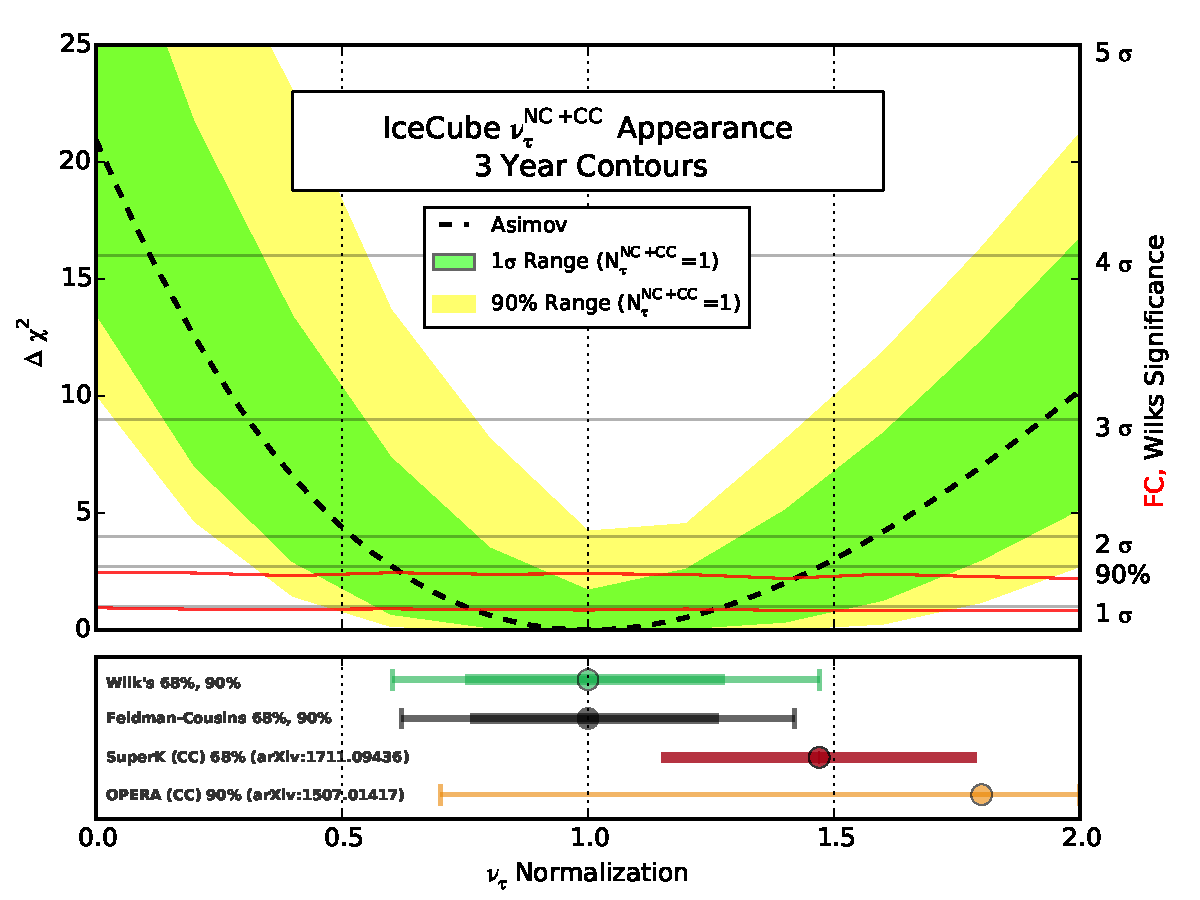
\includegraphics[width=0.48\textwidth]{nc_cc_feldman_cousins.pdf}}
		\subfloat[CC Only]{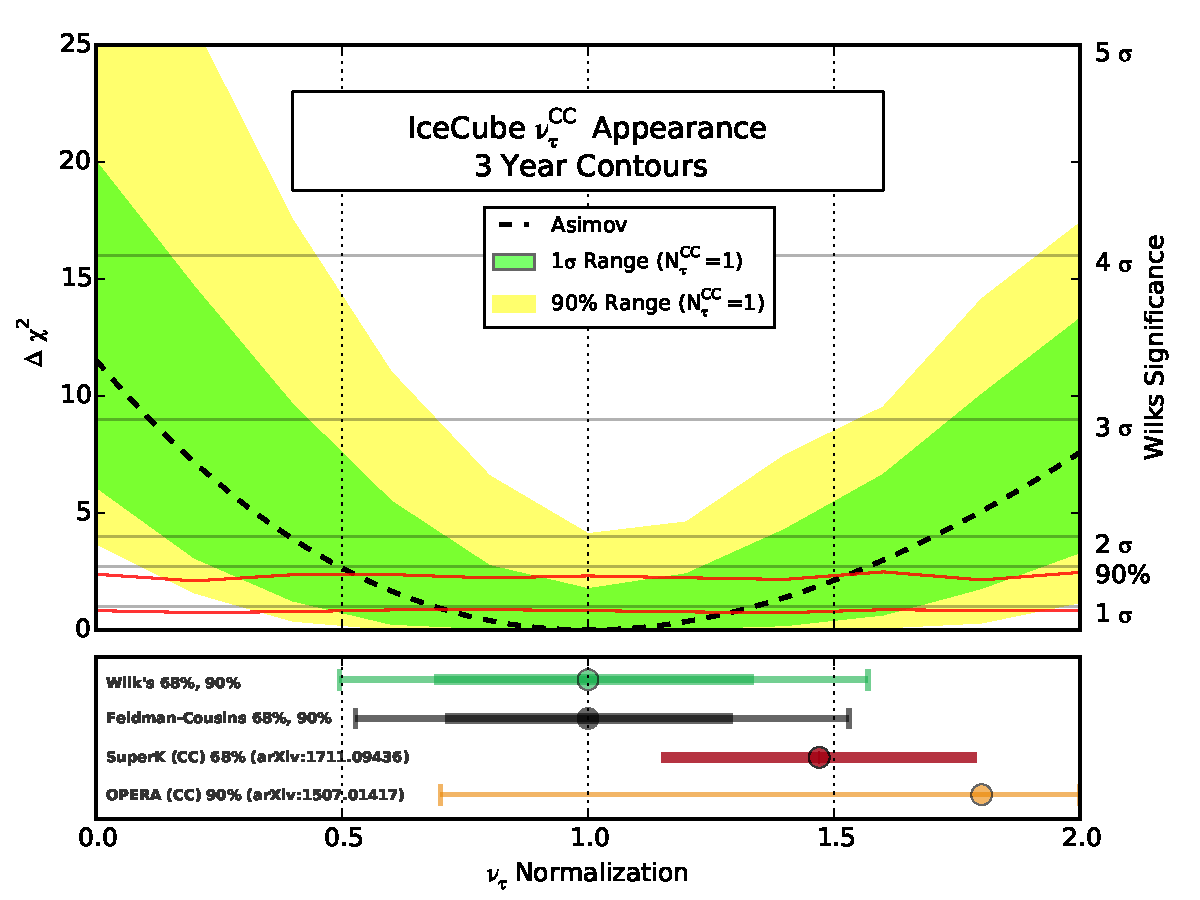
\includegraphics[width=0.48\textwidth]{cc_feldman_cousins.pdf}}
	\caption{The sensitivity of this analysis in the (a) NC+CC and (b) CC-only channel. The top plot shows the Asimov expectation (black dotted line) and the Brazilian flag (green, yellow bands). The significances assuming Wilk's theorem (gray horizontal lines) and Feldman-Cousins (red horizontal lines) are also shown. The bottom plot shows the expected 1$\sigma$ and 90\% ranges for Wilks theorem and Feldman-Cousins compared to the most recent results from the OPERA and Super-Kamiokande analyses.}
	\label{fig:mc_sensitivity}
\end{figure}

The first method, known as the \emph{Asimov} expectation \findref{asimov expectation?}, begins by creating the expected histogram using baseline values of the systematics and oscillations.
The produced histogram, representing an exact PDF of the expected events, is then used as an estimate of the data.
The $\chi^2_{FS}$ is then minimized while the value of $N_{\nu_{\tau}}$ is fixed at regularly spaced points in the interval [0,2] in order to produce a contour.
A final minimization is performed allowing the minimizer to identify the global best-fit value of $N_{\nu_{\tau}}$.

The final expected sensitivity in the Asimov approach is given by calculating the difference between the values of the $\chi^2_{FS}$ at each point and the global best fit.

\begin{equation}
\label{eqn:delta_chi2}
	\Delta \chi^2 \left(N_{\nu_{\tau}}\right) = \chi^2_{FS}\left(N_{\nu_{\tau}}\right)  - \chi^2_{FS}\left(N^{Global}_{\nu_{\tau}}\right)
\end{equation}

The value of $\Delta \chi^2_{FS}$ as a function of $N_{\nu_{\tau}}$ is shown in \needfig{asimov sensitivity}.
These values may be converted into expected significance levels using the procedure described in Section~\ref{subsec:wilks}.

The second method, producing what is known as a \emph{Brazilian flag} plot due to the color scheme, provides an estimate of the expected range of sensitivities in this analysis.
The production of a Brazilian flag begins with the production of a pseudo-data histogram from the Asimov histogram.
Because the simulation sets used here have significant uncertainties due to limited simulation statistics, the first step is to vary the event rate in each bin within the statistical uncertainties of the Monte Carlo.
To do so, histograms of the uncertainty in each bin are produced using the baseline systematics values

\begin{equation}
	\sigma^{MC}_{ijk} = \sqrt{\sum_m^{Evts} w^2_{ijkm}}
\end{equation}

This uncertainty is assumed to be approximately Gaussian.
The event rate in each bin of each simulation template is then varied using a Gaussian distribution using the expected rate as the mean and $\sigma^{MC}$ as the uncertainty.
The new templates are them summed together and each bin is fluctuated around the new expectation assuming Poisson statistics, creating a representation of one possible realization of the data in the analysis.
The OscFit minimization then proceeds as described in the Asimov case using each of 500 realizations of pseudo-data, with the calculation of the $\Delta \chi^2$ as described in \ref{eqn:delta_chi2}.
The Brazilian flag shows the 1$\sigma$ and 2$\sigma$ range of $\Delta \chi^2$ values around the median at each value of $N_{\nu_{\tau}}$.
This provides a graphical representation, shown in \needfig{brazilian flag}, of the expected range of variation of the sensitivity given solely statistical uncertainties.


\label{subsec:wilks}
\subsection{Feldman-Cousins vs WIlk's Theorem}
Estimates of the sensitivity of the analysis were performed using a theorem by Samuel S. Wilks \cite{wilks}.
The theorem gives a statement about the distribution of the likelihood ratio when the likelihoods form a "nested model".
The nested model indicates that the fit parameters used in one fit, ${H_0}$, form a subset of those used in another fit, H.
if the two likelihoods that go into the likelihood ratio differ by N parameters, Wilk's theorem states that the distribution of the test statistic ${-2 ln\left(\frac{L}{L_0}\right)}$ will asymptotically approach a chi-squared distribution with N degrees of freedom.

Wilk's theorem is a powerful tool that may be used to estimate the significances of results and is widely used.
In the case of the measurement of ${\nu_\tau}$ appearance, fits are performed twice in order to obtain the likelihood ratio: once with the value of ${N_\tau}$ fixed to various points and once with ${N_\tau}$ freely floating.
The likelihood ratio is then calculated at each fit point relative to the overall best-fit likelihood using Equation~\ref{eqn:delta_chi2}.
These two fits form a nested model with N=1, allowing the application of Wilk's theorem to estimate significances.

Wilk's theorem gives a useful estimate of the significance and requires negligible additional computational power.
However, the theorem states only an asymptotic limit.
Evaluation of the applicability of Wilk's theorem requires a more robust analysis using Monte Carlo trials.

A more thorough procedure, introduced by Gary Feldman and Robert Cousins \cite{feldman_cousins}, may be applied instead.
Instead of assuming a number of degrees of freedom, the Feldman-Cousins procedure requires directly using the test statistic distribution in order to evaluate the significance.
For public IceCube oscillation results, a method similar to the procedure by Feldman and Cousins is used.

To begin, a value of ${N_\tau^{True}}$ is selected.
Monte Carlo trials are produced with this true value and the likelihood ratio between the best-fit value of ${N_\tau}$ and ${N_\tau^{True}}$ for each trial is calculated.
The distribution of the likelihood ratios is used to identify the value of ${\left(\Delta \chi^2_{FS}\right)}$ below which ${P_{i=1\sigma}\left(\Delta \chi^2_{FS}\right) \approx 68.2689\%}$ of trials lie.
This value is interpreted as the 1${\sigma}$ level for the chosen value of ${N_\tau^{True}}$.
The procedure may be repeated for each required value of ${N_\tau^{True}}$ and different significance levels ${i}$.

Examples of the likelihood ratio distribution for various values of ${N_\tau^{True}}$ are shown in Figure~\ref{fig:llh_ratio_dist}.
A ${\chi^2}$ distribution with 1 degree of freedom is overlaid, showing the expected distribution assuming Wilk's theorem. 
The difference in the 90\% level from Wilks (green) and Feldman-Cousins (red) is also shown.
In general, the distributions show a preference for a slightly narrower distribution than expected from Wilk's theorem.
The difference indicates that the Wilk's theorem approximation may be inaccurate and that the Feldman-Cousins procedure is necessary to correctly characterize the final result.

\begin{landscape}
\begin{figure}
\label{fig:llh_ratio_dist}
\centering 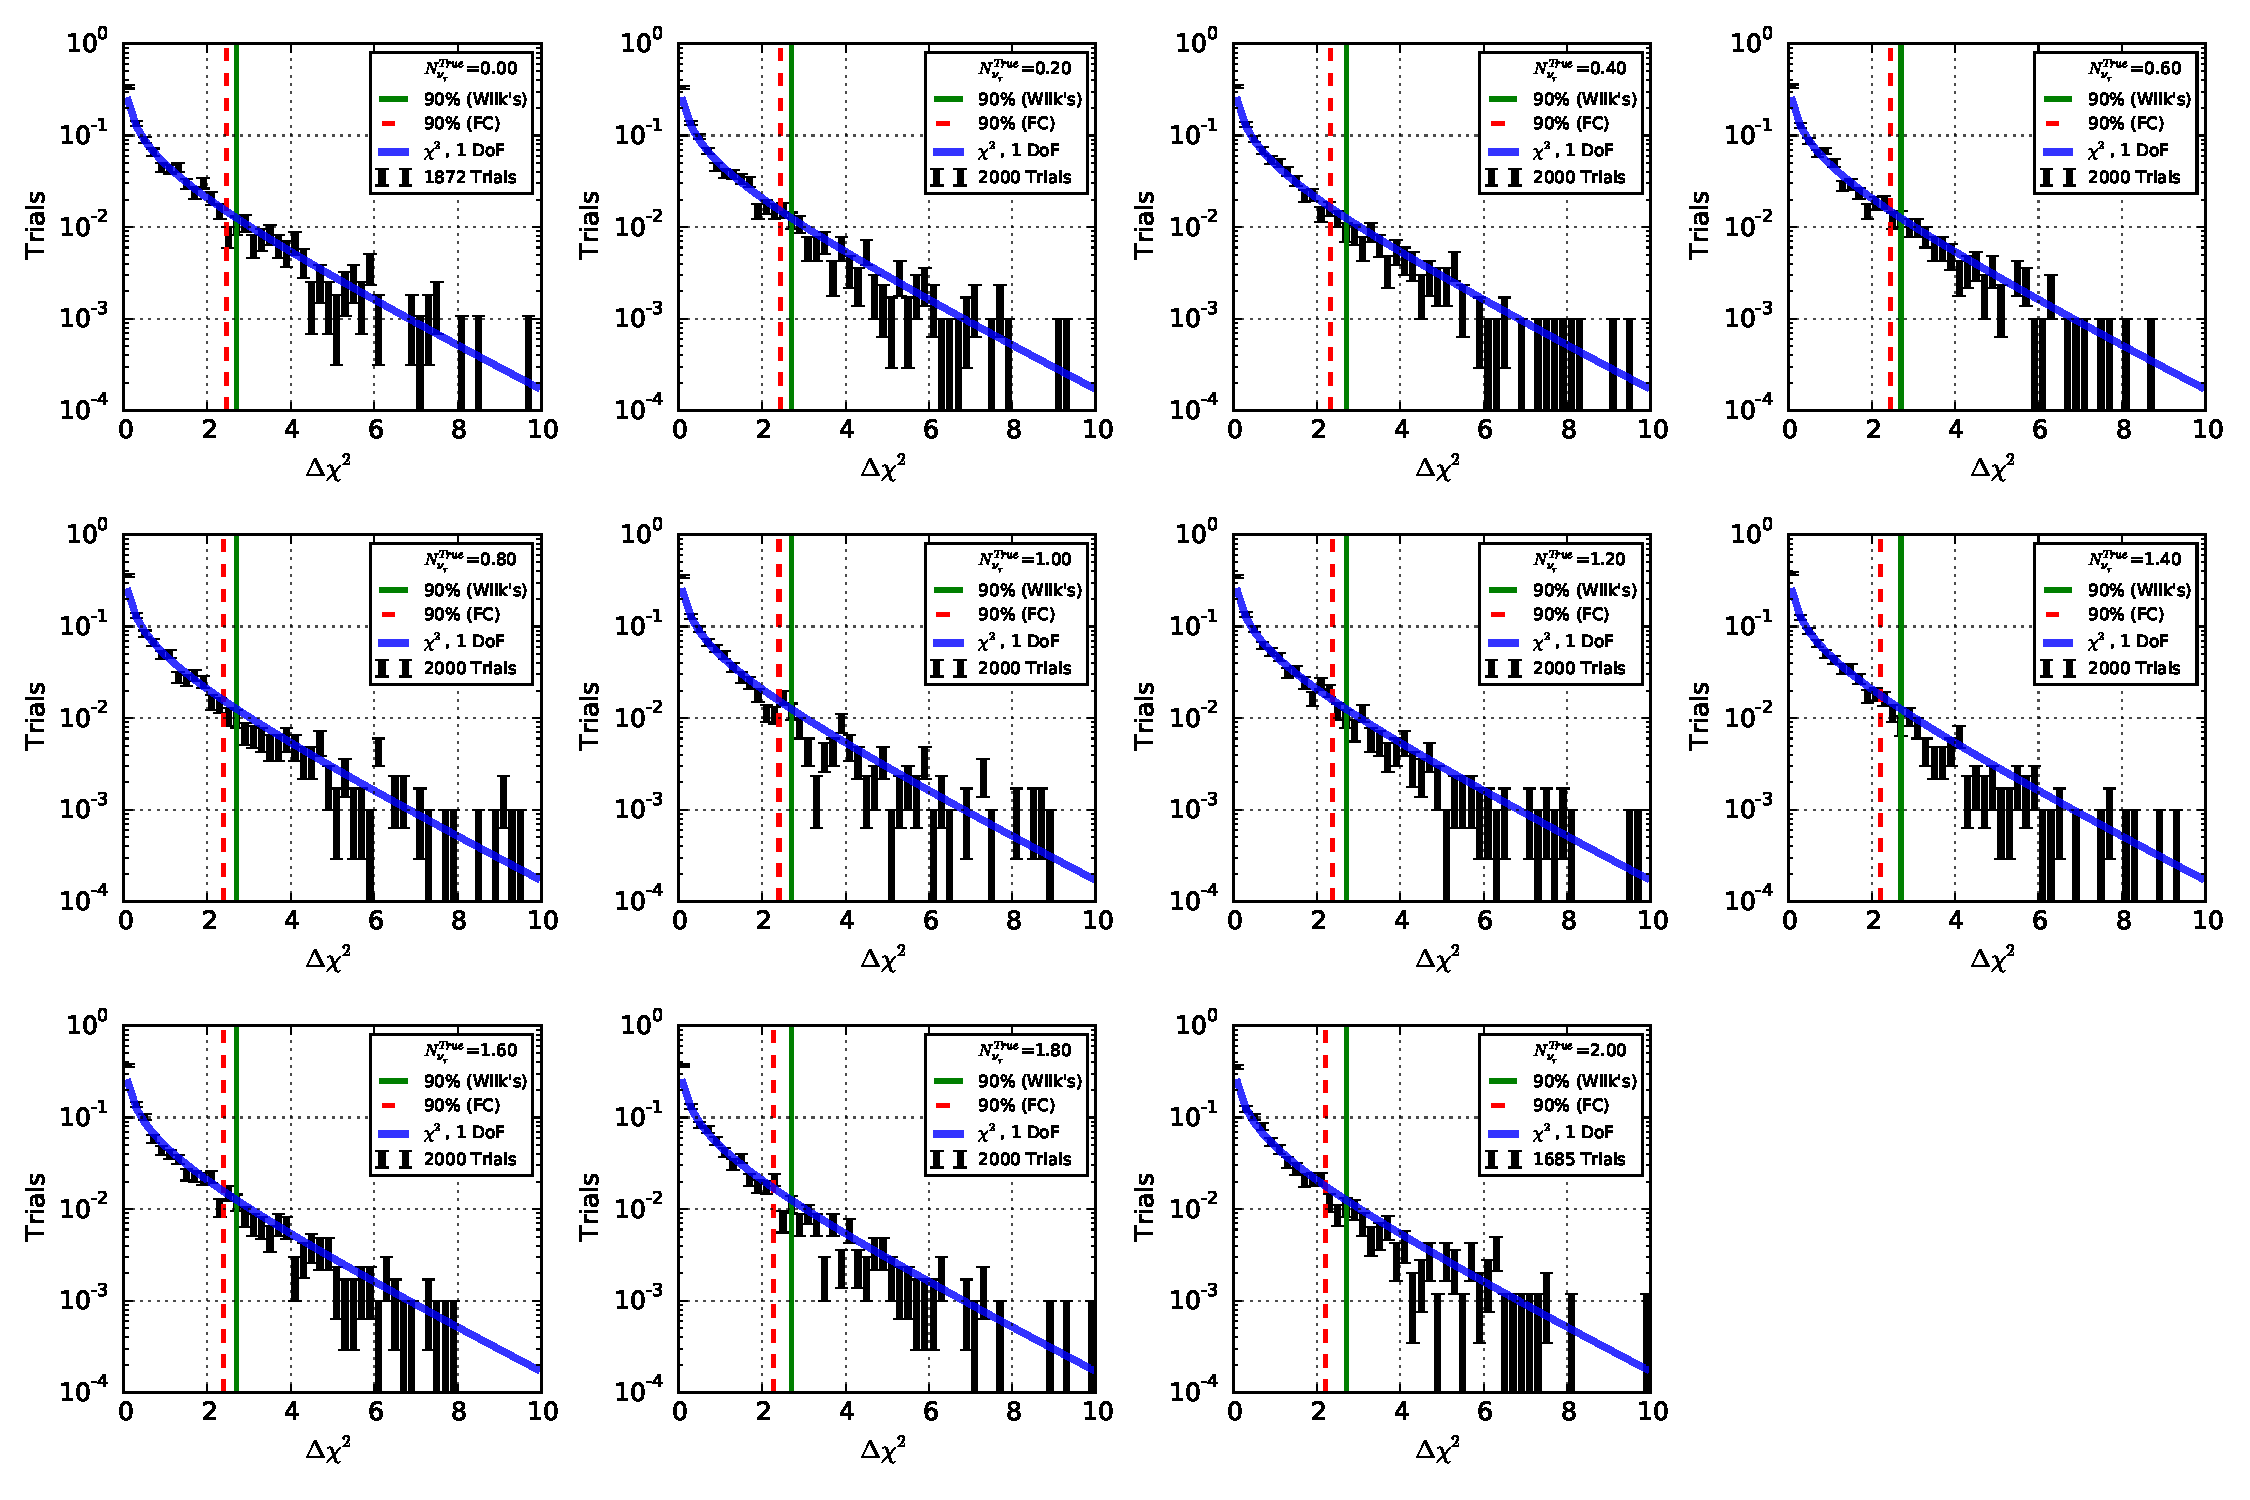
\includegraphics[width=1.2\textwidth]{fc_nc.pdf}
\caption{The test statistic distributions for 11 points in ${N_\tau^{True}}$ in the NC+CC fit. The assumption of 1 degree of freedom from Wilk's theorem is tested by looking at the location of ${\left(\Delta \chi^2_{FS}\right)_{90\%}}$ for each point. The distribution calculated from Monte Carlo trials is narrower than that predicted by Wilk's theorem, indicating that a more complete treatment with the Feldman-Cousins procedure is necessary.}
\end{figure}
\end{landscape}

Once each significance level is obtained for all values of ${N_\tau^{True}}$, a fit to data is performed.
The final confidence intervals at level i are obtained by finding the crossing points between the data contour and the limit obtained for ${P_{i=1\sigma}\left(\Delta \chi^2_{FS}\right)}$, here referred to as ${\left(\Delta \chi^2_{FS}\right)_i}$.

The evaluated ${\left(\Delta \chi^2_{FS}\right)_i}$ are limited to the discrete values chosen in ${N_\tau^{True}}$.
In order to obtain a continuous model, the values of ${\left(\Delta \chi^2_{FS}\right)_i}$ and the contour from data are splined using the UnivariateSpline from Scipy \cite{scipy}.
The crossing points of the two splines may then be calculated to obtain the best estimate for the final result.

The procedure does not rely on assumptions about the test statistic distribution and works even in cases where the likelihood ratio distribution does not chi-squared distributed.
The number of trials required to reduce the effect of statistical fluctuations in the evaluation, however, can make such evaluations prohibitively expensive.
In order to evaluate the 90\% confidence interval at 10 points from ${0 \leq N_\tau^{True} \leq 2}$ with minimal fluctuation requires on the order of 1000 trials at each point.
Higher significance levels may increase the number of trials required exponentially.
Each of these 10,000 trials must be fit a total of four times: each combination of ${N_\tau}$ free/fixed and each of the two octants in ${sin^2 \theta_{23}}$ must be tested separately.
The procedure must be run separately for the CC-only and NC+CC fits, doubling the computational resources required.
At approximately one hour per fit, this leads to a requirement of approximately 10 CPU-years worth of computing power. 

Any changes to the analysis, including additional cuts and systematics changes, may lead to differences in the values of ${\left(\Delta \chi^2_{FS}\right)_i}$.
In order to reduce the total computation power required for tests in this analysis, the full Feldman-Cousins procedure as described here was only applied once the final result was unblinded.
Until that point, all significances were calculated assuming Wilk's theorem.

\label{subsec:systematics_impact}
\subsection{Impact of Systematics}
There are various ways to measure the impact of the included systematics in this analysis.
Described here are methods to evaluate, in order of increasing importance, the total systematics impact, the impact of each systematic individually, the correlation between systematics, and the effect of non-baseline values.
Each of these test different aspects of the sensitivity and all are included for completeness.

\subsubsection{Total Systematics Impact}
The total impact of the systematics on the sensitivity may be measured by comparing the total Asimov sensitivity to an Asimov sensitivity calculated using no systematics.
This is shown in \needfig{comparison of stat-only fit to full systematics fit}.
It is clear from the comparison that the analysis is very sensitive to the included systematics set.

\subsubsection{N+1 Tests: Sensitivity of Analysis to Systematic}
A different test is also possible: Instead of calculating likelihoods with no systematics included, a single systematic may be used at a time.
This test, called an N+1 test for the addition of one systematic at a time, yields useful information on a sample's sensitivity to single systematics.
A small change in sensitivity between the no-systematics case above and an N+1 Asimov sensitivity may have two possible explanations.
The first that the current analysis is unaffected by changes in the systematic, implying that the systematic may be investigated for removal in the analysis.
The second possibllity is that the systematic may interact with other parameters in order to produce an effect.
The second case is more difficult to diagnose, but further tests may be possible.
\needfig{N+1 tests}

\subsubsection{N-1 Tests: Redundancy Between Systematics}
In contrast to the N+1 tests, N-1 tests start with the full suite of systematics included.
One systematic is then fixed to the baseline value and removed before redoing minimization.
The change in the contour as a result of the removal of systematics allows for the investigation of redundancy between systematics.
If, for example, two systematics have similar effects in the final histogram, then the N-1 test will show no change in sensitivity due to the removal.
It is also possible that the analysis is strongly sensitive to the value of the systematic and is unlikely to move from the baseline value.
These tests can be useful in identifying redundant parameters for removal, although with the caveat that combinations of parameters are not tested.
After removal of multiple redundant parameters, the updated Asimov sensitivity should be tested once again to verify that the combination of removed parameters remains irrelevant for the fit

\needfig{N-1 tests}

\subsubsection{"Hidden Potential" Tests: Non-Baseline Values}
Both the N+1 and N-1 test suffer from a particular flaw.
Both fail to test the analysis for exceptionally strong sensitivity to particular systematics.
In order to identify these parameters, the "hidden potential" test has been proposed.
In this test, the Asimov sensitivity of the full analysis containing all proposed systematics is used as a baseline.
Each systematic is then fixed, one at a time, off of the baseline value before rerunning the minimization.
The parameters with priors tend to be fixed to one standard deviation from the prior mean.
The change in the sensitivity gives an indirect measure of the strength of the systematic effect in the analysis.
If no change is observed, the parameter is likely to be redundant and may be investigated for removal from the analysis.

\needfig{hidden potential martin n-1 tests}.
\unsure{should i be including the dropped dis/theta13 systematics here? and maybe deltacp? otherwise this section feels a bit pointless}

